\documentclass[orivec]{llncs}
\usepackage{graphicx}
\usepackage{amsmath}			% for "cases"
\usepackage{amsfonts}		% for frakur fonts
\usepackage{mathrsfs}		% for curly "E" error symbol
\usepackage{float}
\usepackage{tcolorbox}		% for wrapping example in color box
\usepackage{wrapfig}			% wrap figure beside text, used in example
\usepackage{tikz-cd}			% commutative diagrams
\usepackage{amssymb}			% for \multimap, \updownarrow, \bigstar
\usepackage{sectsty}			% change section color
\usepackage{turnstile}		% longer turnstiles
\usepackage{hyperref}		% include web link for RL sample code

\usepackage{geometry}		% change paper size
\geometry{
  a4paper,         % or letterpaper
  textwidth=18cm,  % llncs has 12.2cm
  textheight=27cm, % llncs has 19.3cm
  heightrounded,   % integer number of lines
  hratio=1:1,      % horizontally centered
  vratio=2:3,      % not vertically centered
}
\usepackage[fontsize=13pt]{scrextend}

% *************** Delete when not using Chinese or colors **********************
\usepackage{xeCJK}
\setCJKmainfont[BoldFont=SimHei,ItalicFont=KaiTi]{SimSun}
\usepackage{color}
\definecolor{Cerulean}{RGB}{100,100,200}
\newcommand{\emp}[1]{\textbf{\textcolor{Cerulean}{#1}}}
\definecolor{grey}{rgb}{0.9,0.9,0.9}  % grey

% \chapterfont{\color{blue}}  % sets colour of chapters
\sectionfont{\color{blue}} 
\subsectionfont{\color{blue}} 
\subsubsectionfont{\color{blue}} 

\newcommand{\vect}[1]{\boldsymbol{#1}}
\newcommand*\sigmoid{\vcenter{\hbox{
\includegraphics{sigmoid.png}}}}
\newcommand*\KB{\vcenter{\hbox{
\includegraphics{KB-symbol.png}}}}
\newcommand*\invsigmoid{\vcenter{\hbox{
\includegraphics{inverse-sigmoid.png}}}}
\newcommand{\invW}{\, \rotatebox[origin=c]{90}{W}}
\newcommand{\invw}{\, \rotatebox[origin=c]{90}{w}}
\newcommand*\rectifier{\vcenter{\hbox{
\includegraphics{rectifier.png}}}}
\newcommand{\dashh}{\textemdash~}
\newcommand{\code}[1]{{\footnotesize{\ttfamily #1}}}
\newcommand{\tab}{\hspace*{1cm} }

% ***** Boxed variables inside math equations
% \newcommand*{\boxedcolor}{black}
\makeatletter
% \renewcommand{\boxed}[1]{\textcolor{\boxedcolor}{%
% \fbox{\normalcolor\m@th$\displaystyle#1$}}}
% \setlength{\fboxsep}{1pt}
\renewcommand{\boxed}[1]{\fbox{\m@th$\displaystyle\scalebox{0.9}{#1}$} \,}
\makeatother

\overfullrule=0mm

\newsavebox{\MyName}
\savebox{\MyName}{
\includegraphics[scale=0.6]{YKY.png}}

\title{控制论 tutorial}
\titlerunning{控制论 tutorial}
\author{\usebox{\MyName} (King-Yin Yan)
% \\ \footnotesize{General.Intelligence@Gmail.com}
}
\institute{General.Intelligence@Gmail.com}

\begin{document}

\maketitle
\setlength{\parindent}{0em}
% \setlength{\parskip}{2.8ex plus0.8ex minus0.8ex}
\setlength{\parskip}{2.8ex}

\section{控制论}

以下内容可以在一般「现代控制论」教科书中找到,例如:
\let\labelitemi\labelitemii
\begin{itemize}
\item Daniel Liberzon 2012: \textit{Calculus of variations and optimal control theory -- a concise introduction}
\item 李国勇 2008: 《最优控制理论与应用》
\item 张洪钺、王青 2005: 《最优控制理论与应用》
\end{itemize}

一个\emp{动态系统 (dynamical system)} 可以用以下方法定义:
\begin{eqnarray}
\mbox{离散时间:} \quad \quad & \vect{x}_{t+1} = \vect{F}(\vect{x}_t) \\
\mbox{连续时间:} \quad \quad & \dot{\vect{x}} = \vect{f}(\vect{x}) \label{eqn1}
\end{eqnarray}
其中 $f$ 也可以随时间改变。 如果 $f$ 不依赖时间,则系统是 time-invariant (定常的),形式上如(\ref{eqn1}) 那种微分方程叫作 autonomous (自主的)。

在我的智能系统理论里,我把 $F$ 或 $f$ 设定成 RNN (recurrent neural network),即反馈式神经网络:
\begin{eqnarray}
\mbox{离散时间:} \quad \quad & \vect{x}_{t+1} = \boxed{\mbox{RNN}}(\vect{x}_t) \\
\mbox{连续时间:} \quad \quad & \dot{\vect{x}} = \boxed{\mbox{RNN}}(\vect{x})
\end{eqnarray}
这里 recurrent 指的是它不断重复作用在 $\vect{x}$ 之上,但实际上它是一个普通的前馈式 (feed-forward) 神经网络。 注意: 在抽象理论中,$f$ 和 $F$ 可以是任意函数,我把它们设计成 NN 只是众多可能的想法之一。 之所以选用 NN,是因为它有 universal function approximator 的功能,而且是我们所知的最「聪明」的学习机器之一。

在我提出的智能系统里,$\dot{x}$ 是由\emp{學習機器}給出的,換句話說,$\dot{x}$ 是思維狀態在梯度下降至最佳狀態時的\emp{方向導數}。

一个(连续时间的)\emp{控制系统 (control system)} 定义为:
\begin{equation}
\dot{\vect{x}}(t) = f(\vect{x}(t), \vect{u}(t), t)
\end{equation}
其中 $\vect{u}(t)$ 是\emp{控制向量}。 控制论的目的就是找出最好的 $\vect{u}(t)$ 函数,令系统由初始状态 $\vect{x}_0$ 去到终点状态 $\vect{x_\bot}$。

注意: 人工智能中的 \emp{A* search},是动态规划的一个特例。 换句话说,用动态规划在某个空间中「漫游」,可以模拟到 best-first 搜寻的功能。

在这框架下,智能系统的运作可以分开成两方面: \emp{思考} 和 \emp{学习}。

\emp{思考}即是根据已学得的知识(知识储存在 RNN 里),在思维空间中找寻 $\vect{x}$ 最优的轨迹,方法是用控制论计算 $\vect{u}^*$。 $\vect{x}$ 的轨迹受 RNN 约束(系统只能依据「正确」的知识去思考),但思考时 RNN 是不变的。

\emp{学习}就是学习神经网络 RNN 的 weights $W$。 此时令 $u = 0$,即忽略控制论方面。

以上两者是两个独立的方面,但不排除它们可以在实际中同时进行。

\subsection{控制论与强化学习的关系}

在\emp{强化学习}中,我们关注两个数量:
\let\labelitemi\labelitemii
\begin{itemize}
\item $R(\vect{x},a)$ = 在状态 $\vect{x}$ 做动作 a 所获得的\emp{奖励}(reward)
\item $U(\vect{x})$ = 状态 $\vect{x}$ 的\emp{效用}(utility) 或 \emp{价值} (value) % 或 $V(\vect{x})$
\end{itemize}
简单来说,「价值」就是每个瞬时「奖励」对时间的积分:
\begin{equation}
\boxed{\mbox{价值} U} = \int \boxed{\mbox{奖励} R} \,dt
\end{equation}
(价值有时用 $V$ 表示,但为避免和势能 $V$ 混淆故不用。)

用\emp{控制论}的术语,通常定义 cost functional:
\begin{equation}
J = \int L dt + \Phi(\vect{x}_\bot)
\end{equation}
其中 $L$ 是 ``running cost'',即行走每一步的「价钱」; $\Phi$ 是 terminal cost,即到达终点 $\vect{x}_\bot$ 时,那位置的价值。

%Define a continuous version of ``utility'':
%\begin{equation}
%V(x,t) = \min_u \{ \int_t^{t_\bot} C(x,u)dt + \Phi(x_\bot,t_\bot) \} 
%\end{equation}
%where $t$ is time, $u$ is a set of control parameters, $C$ is the \emp{cost-rate} function:
%\begin{equation}
%\int C dt = R = \mbox{reward}
%\end{equation}
%This integral expresses the ``cost of the path'', whereas $\Phi(x_\bot,t_\bot)$ is the ``cost at termination''.

在\emp{分析力学}里 $L$ 又叫 Lagrangian,而 L 对时间的积分叫「作用量」:
\begin{equation}
\boxed{\mbox{作用量 (Action)}} \; S = \int L dt
\end{equation}
Hamilton 的\emp{最小作用量原理} (principle of least action) 说,在自然界的运动轨迹里,$S$ 的值总是取稳定值 (stationary value),即比起邻近的轨迹它的 $S$ 值最小。

所以有这些对应:\\
\begin{center}
\begin{tabular}{|c|c|c|}
\hline 
\emp{强化学习} & \emp{最优控制} & \emp{分析力学} \\ 
\hline
效用/价值 $U$ & 价钱 $J$ & 作用量 $S$ \\ 
\hline 
即时奖励 $R$ & running cost & Lagrangian $L$ \\ 
\hline 
action $a$ & control $u$ & (外力?) \\
\hline
\end{tabular} 
\end{center}

用比较浅显的例子: 和美女做爱能带来即时的快感 (= 奖励 $R$),但如果强奸的话会坐牢,之后很长时间很苦闷,所以这个做法的长远价值 $U$ 比其他做法较低,正常人不会选择它。

有趣的是,奖励 $R$ 对应於力学上的 Lagrangian,其物理学单位是「能量」; 换句话说,「快感」或「开心」似乎可以用「能量」的单位来量度,这和通俗心理学里常说的「正能量」不谋而合。 而,长远的价值,是以 $[\mbox{能量} \times \mbox{时间}]$ 的单位来量度。

一个智能系统,它有「智慧」的条件,就是每时每刻都不断追求「开心能量」或奖励 $R$ 的最大值,但它必需权衡轻重,有计划地找到长远的效用 $U$ 的最大值。

\subsection{经典分析力学(analytical mechanics)}

分析力学的物理内容,完全是牛顿力学的 $F = ma$,但在表述上引入了能量和 Hamiltonian 等概念,再使用微积分和变分法。

\subsubsection{Lagrange 方程}

Lagrange 引入了 Lagrangian $L = T - V$,可以分拆成\emp{動能} $T$ 和\emp{勢能} $V$ 兩部分。

重點是: \emp{動能} $T$ 是速度 $\dot{\vect{x}}$ 的函數,\emp{勢能} $V$ 是位置 $\vect{x}$ 的函數。

问题: 如果在强化学习中的「快感/奖励」对应於 Lagrangian $L$,如何在奖励之中分拆出「动能」和「势能」的分量? 

\begin{equation}
\boxed{\mbox{Lagrange equation}} \quad
\frac{d}{dt} \frac{\partial L}{\partial \dot{x}_i} - \frac{\partial L}{\partial x_i} = 0
\end{equation}
这些方程的座标是 $(\vect{x}, \dot{\vect{x}})$,可以了解成\emp{位置空间 (configuration space)}上的 tangent bundle (下述)。

\subsubsection{Hamilton 方程}

\emp{Hamiltonian} $H = T + V$,亦即总能量,但它表示成位置 $\vect{x}$ 和动量 $\vect{p}$ 的函数。

\begin{equation}
\label{Hamilton-eqns}
  \boxed{\mbox{Hamilton equation}} \quad
  \begin{cases}
      \dot{\vect{x}} & = \displaystyle \frac{\partial H}{\partial p} \\
      \dot{\vect{p}} & = - \displaystyle \frac{\partial H}{\partial x}
  \end{cases}
\end{equation}
这些方程的座标是\emp{相位空间 (phase space)} $(\vect{x}, \vect{p})$。

位置空间和相位空间之间的变换是 \emp{Legendre transformation}:
\begin{eqnarray}
\boxed{\mbox{tangent bundle}} \; T X & \rightarrow & T^* X \; \boxed{\mbox{cotangent bundle}} \\
(\vect{x}, \dot{\vect{x}}) & \mapsto & (\vect{x}, \vect{p})
\end{eqnarray}
\begin{equation}
\vect{p} = \frac{\partial L}{\partial \dot{\vect{q}}} \quad \Rightarrow \quad H := \vect{p} \dot{\vect{x}} - L
\end{equation}

\subsubsection{Hamilton-Jacobi 方程}

\begin{equation}
\boxed{\mbox{Hamilton-Jacobi equation}} \quad
H(q, \frac{\partial S}{\partial q}, t) + \frac{\partial S}{\partial t} = 0
\end{equation}
其中 $S$ 是「作用量」。 下面我们会用动态规划的原理推导出此一方程。

\subsubsection{Poisson 括号}

\begin{equation}
\label{Poisson-bracket}
\boxed{\mbox{Poisson 括号}} \quad \{ F, H \} := \sum_i \{ \frac{\partial F}{\partial q_i} \frac{\partial H}{\partial p_i} - \frac{\partial F}{\partial p_i} \frac{\partial H}{\partial q_i} \}
\end{equation}
在力学系统中,它表示任意一力学量(函数 $f$)对时间的改变量:
\begin{equation}
\dot{f} = \{ f, H \} 
\end{equation}
\begin{equation}
\frac{\partial}{\partial t} = \frac{\partial}{\partial p} \dot{p} + \frac{\partial}{\partial q} \dot{q}
\end{equation}
以上使用了微分的 chain rule,但由於 $\dot{\vect{p}}$ 和 $\dot{\vect{q}}$ 可以由 Hamilton 方程 (\ref{Hamilton-eqns}) 给出,所以得到 Poisson 括号的形式 (\ref{Poisson-bracket})。

每个物理学生都知道的「经典-量子对应原理」:
\begin{equation}
[\vect{F}, \vect{G}] \quad \Leftrightarrow \quad i \hbar \{ F, G \}
\end{equation}
这对应原理是 P.A.M. Dirac 发现的。

在经典力学里,
\begin{equation}
\{ \vect{x}, \vect{p} \} = 1
\end{equation}
但在量子力学里,
\begin{equation}
[ \vect{X}, \vect{P} ] = i \hbar
\end{equation}
这也是 Heisenberg 测不准原理的由来:
\begin{equation}
\Delta \vect{X} \Delta \vect{P} \ge \frac{\hbar}{2}
\end{equation}

如果在某一流形上,「广义」Poisson 括号是 nondegenerate (非退化)的,则它变成了\emp{辛流形}结构的 $\omega = \{ \cdot, \cdot \}$ 括号 (下述)。

\subsection{Hamiltonian 的出现}

考虑一个典型的控制论问题,系统是:
\begin{eqnarray}
\mbox{状态方程:} \quad & \dot{\vect{x}}(t) = \vect{f}[\vect{x}(t), \vect{u}(t), t] \\
\mbox{边值条件:} \quad & \vect{x}(t_0) = \vect{x}_0 \,,\, \vect{x}(t_\bot) = \vect{x}_\bot \\
\mbox{目標函数:} \quad & J = \int_{t_0}^{t_\bot} L[\vect{x}(t), \vect{u}(t), t] dt
\end{eqnarray}
要找的是最优控制 $\vect{u}^*(t)$。

\begin{figure}[H]
\begin{center}
\colorbox{grey}{\parbox{0.95\textwidth}{\setlength{\parskip}{2.5ex}

\emp{Lagrange multiplier} 是找极大/小值的常用方法: 如果我们要找:
\begin{equation}
\max \; f(x) \quad \mbox{ subject to } \quad g(x) = 0
\end{equation}
Lagrange 建议我们建构 Lagrangian 函数:
\begin{equation}
L(x, \lambda) = f(x) - \lambda g(x)
\end{equation}
然后求解:
\begin{equation}
\nabla_{x,\lambda} L = 0
\end{equation}
}}
\end{center}
\end{figure}

现在将 Lagrange multiplier 方法应用到我们的问题上,会发现新的目标函数是:
\begin{equation}
J = \int_{t_0}^{t_\bot} \{ L + \vect{\lambda}^T(t) \left[ f(\vect{x}, \vect{u}, t) - \dot{\vect{x}} \right] \} dt
\end{equation}
因此可以引入一个新的标量函数 $H$,即 Hamiltonian:
\begin{equation}
H(\vect{x}, \vect{u}, t) = L(\vect{x}, \vect{u}, t) + \vect{\lambda}^T(t) f(\vect{x}, \vect{u}, t)
\end{equation}
物理学上,$\vect{f}$ 的单位是速度,而 $L$ 的单位是能量,所以 $\vect{\lambda}$ 应该具有 \emp{动量} 的单位。

\subsubsection{极小值原理}

Lev Pontryagin (1908-1988) 提出了 \emp{极小值原理},是经典变分法的推广。 经典变分法的最优条件是:
\begin{equation}
\frac{\partial H}{\partial \vect{u}} = \vect{0}
\end{equation}
极小值原理将最优条件改成是:
\begin{equation}
\min_{u \in \Omega} H(\vect{x}^*, \vect{\lambda}^*, \vect{u}, t) = H(\vect{x}^*, \vect{\lambda}^*, \vect{u}^*, t)
\end{equation}
即是说: 在最优轨迹 $\vect{x}^*(t)$ 和最优控制 $\vect{u}^*(t)$ 上,$H$ 取最小值。 它的好处是,当 $\displaystyle \frac{\partial H}{\partial \vect{u}}$ 不连续或不存在时,或者 $\vect{u}$ 受其他约束时,也可以应用。

粗略来说,极小值原理比经典变分法更一般,而动态学习又比极小值原理更一般。

\subsubsection{Hamilton-Jacobi-Bellman 方程}

\begin{itemize}
\item Stanislaw Zak (2003): \textit{Systems and control}
\end{itemize}

% \S 5.4.3 Zak.

用动态规划的 \emp{Bellman optimality condition} 可以推导出微分形式的 Hamilton-Jacobi-Bellman 方程。  重温一下,Bellman 最优条件说的是: 「从最优路径末端切去一小截之后,馀下的还是最优路径。」  它通常写成如下的 recursive 形式:
\begin{eqnarray}
\boxed{\mbox{最优路径}} & = & \mbox{在小段上选取最大奖励} + \boxed{\mbox{馀下的最优路径}} \\
J^*_t & = & \max_{u} \{ \boxed{\mbox{奖励}(u, t)} + J^*_{t-1} \}
\end{eqnarray}

\begin{equation}
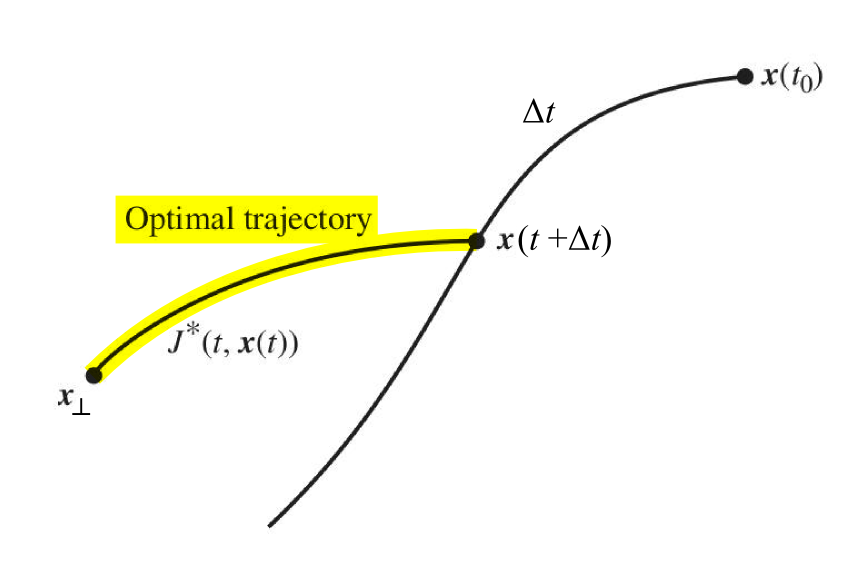
\includegraphics[scale=0.4]{optimal-trajectory.png}
\end{equation}

我们在时间 interval 的开端切出一小段:
\begin{equation}
[ t_0, t_\bot ] = [ t_0, t_0 + \Delta t ] \cup [ t_0 + \Delta t, t_\bot ]
\end{equation}
我们想优化的目标函数是:
\begin{equation}
J^*(t, \vect{x}, \vect{u}) = \min_u \{ \int_{t_0}^{t + \Delta t} L d\tau + \int_{t + \Delta t}^{t_\bot} L d\tau + \Phi(t_\bot, \vect{x}_\bot) \}
\end{equation}
根据 Bellman 条件,目标函数变成:
\begin{equation}
J^*(t, \vect{x}) = \min_u \{ \int_{t_0}^{t + \Delta t} L d\tau + J^*(t + \Delta t, \vect{x}(t + \Delta t)) \}
\end{equation}
用 Taylor series 展开右面的 $J^*$:
\begin{equation}
J^* + \frac{\partial J^*}{\partial t} \Delta t + \frac{\partial J^*}{\partial \vect{x}}(\vect{x}(t + \Delta t) - \vect{x}(t)) + \mbox{H.O.T.}
\end{equation}
左右两边的 $J^*$ 互相消去,而且 $\vect{x}(t + \Delta t) - \vect{x}(t) \approx \dot{\vect{x}} \Delta t$,於是有:
\begin{equation}
0 = \min_u \{ \int_{t_0}^{t + \Delta t} L d\tau + \frac{\partial J^*}{\partial t} \Delta t + \frac{\partial J^*}{\partial \vect{x}} \dot{\vect{x}} \Delta t + \mbox{H.O.T.} \}
\end{equation}
又由於 $\Delta t$ 很小,而且 $\dot{\vect{x}} = \vect{f}$,所以:
\begin{equation}
0 = \min_u \{ L \Delta t + \frac{\partial J^*}{\partial t} \Delta t + \frac{\partial J^*}{\partial \vect{x}} \vect{f} \Delta t + \mbox{H.O.T.} \}
\end{equation}
全式除以 $\Delta t$ 并令 $\Delta t \rightarrow 0$:
\begin{equation}
0 = \frac{\partial J^*}{\partial t} + \min_u \{ L + \frac{\partial J^*}{\partial \vect{x}} \vect{f} \}
\end{equation}
记得 Hamiltonian 的定义是 $\displaystyle H = L + \frac{\partial J^*}{\partial \vect{x}} \vect{f}$,所以得到想要的结果:
\begin{equation}
\boxed{\mbox{Hamilton-Jacobi equation}} \quad
0 = \frac{\partial J^*}{\partial t} + \min_u H
\end{equation}

% The differential version is the Hamilton-Jacobi equation:
% \begin{equation}
% \frac{d}{dt} V(x,t) = \min_u \{ C(x,u) + \langle \nabla V(x,t), f(x,u) \rangle \} 
% \end{equation}
% where $x$ must obey this dynamics:
% \begin{equation}
% \dot{x}(t) = f(x(t),u(t)).
% \end{equation}

这个方程和量子力学中的 \emp{Schr\"{o}dinger equation} 很相似:
\begin{equation}
i \hbar \frac{\partial}{\partial t} \Psi(x,t) = \left[ V(x,t) + \frac{-\hbar^2}{2\mu} \nabla^2 \right] \Psi(x,t).
\end{equation}
其中 $\Psi$ 类似於我们的 $J$ (或许 $\Psi$ 是自然界希望取极值的某种东西?)

\subsection{Symplectic 结构}

\begin{itemize}
\item Stephanie Singer (2001): \textit{Symmetry in mechanics -- a gentle, modern introduction}
\item 锺万勰 2011: 《力、功、能量与辛数学》
\end{itemize}

Symplectic 的拉丁文意思是「互相交错 (intertwined)」,它用来描述 Hamiltonian 系统的几何结构。 中文译作「辛」是音译。  Symplectic 概念是 Hermann Weyl 研究 Hamilton 系统的对称性时在 1939 年提出的。

在数值计算上,处理 Hamilton 系统时,如果算法尊重 symplectic 结构(叫 symplectic integrators),会比一般的算法更准确; 而一般解微分方程的算法,例如 Euler 算法和 Runge-Kutta 算法,有时会给出错误的结果。

举例来说,从 Hamiltonian 的角度来看,动量 $p$ (momentum) 和 速度 $v$ (velocity) 是成\emp{对偶}的,$p$ 总是伴随 $v$ 出现,因为 $p \cdot v = mv^2$ 的单位是能量。

举另一个例子,假设我们有两个用来定义系统状态的向量:
\begin{equation}
x_1 = \left(
\begin{array}{c}
s_1\\
f_1\\
\end{array}
\right), \quad
x_2 = \left(
\begin{array}{c}
s_2\\
f_2\\
\end{array}
\right)
\end{equation}
其中 $s$ 是位移(单位是长度),$f$ 是力。 这两个向量的「辛内积」定义为:
\begin{eqnarray}
\langle x_1, x_2 \rangle & = & x_1^T \, J \, x_2 \nonumber \\
& = &
\left(
\begin{array}{c}
s_1\\
f_1\\
\end{array}
\right)^T
\left( \begin{array}{cc}
0  & I \\
-I & 0 \end{array} \right)
\left(
\begin{array}{c}
s_2\\
f_2\\
\end{array}
\right) \\
& = & f_2 s_1 - f_1 s_2 \nonumber
\end{eqnarray}
其中矩阵 $J$ 就是辛的微分形式 $\omega$ 的结构矩阵(下述)。 由於 $f \cdot s$ 表示的是「所做的功」,上式表示的是
\begin{multline}
(\mbox{状态1的力对状态2的位移所做的功}) - \\
(\mbox{状态2的力对状态1的位移所做的功})
\end{multline}
也就是「相互功」,辛正交则 $\langle x_1, x_2 \rangle = 0$,代表 work reciprocity(功的互等),所以辛几何是一种关於能量的代数。

在微分几何里,研究抽象的 Hamiltonian systems,会发现 symplectic 结构。 这结构用微分流形 $M$ 及其上的一个 微分形式 (differential form) $\omega$ 来定义。 需要一些微分几何的基础.....

\subsubsection{Vectors and co-vectors}

Vector 和 co-vector 之间的关系,可以看成是「$d$ 别人的东西」和「被别人 $d$ 的东西」,这里 $d$ 表示微分。

「$d$ 别人的东西」是线性的 differential operators,记作 $\displaystyle \frac{\partial}{\partial x_1}$、$\displaystyle \frac{\partial}{\partial x_2}$ 等;它们很自然地组成一个 vector space $T_x M$。

「被别人 $d$ 的东西」是一些线性的微分形式,记作 $dx_1$、$dx_2$ 等; 它们属於 $T_x M$ 的 dual space。

\subsubsection{Manifolds}

基本上「流形」的意思是「弯曲的空间」,它们局部地近似於 Euclidean 空间 $\mathbb{R}^n$,局部的座标可以分段用一组微分映射来描述,这些 maps 叫 charts。
\begin{equation}
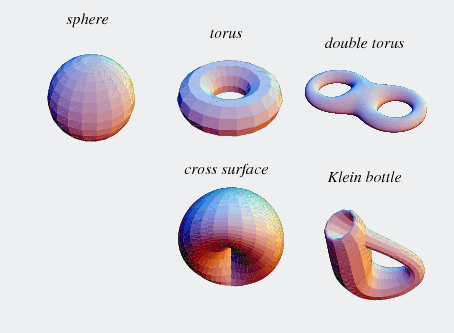
\includegraphics[scale=0.5]{smooth-manifolds.png}
\end{equation}

\subsubsection{Phase space}

「相位空间」指的是力学系统里,$i$ 个粒子的位置 $x_i$ 和动量 $p_i$ 合并而成的 $(\vect{x}, \vect{p})$ 空间。 但 configuration space 指的是所有可容许的位置 $\vect{x}$ 的空间。

\subsubsection{Vector fields, differential forms, Hamiltonian flow}

根据 Hamilton 方程,再用微分的 chain rule 可以得到:
\begin{equation}
\frac{d}{dt} = \frac{\partial H}{\partial \vect{p}} \frac{\partial}{\partial \vect{x}} - \frac{\partial H}{\partial \vect{x}} \frac{\partial}{\partial \vect{p}}
\end{equation}
它是一个微分算子,亦即是\emp{向量场}; 它有个特别的名字叫 Hamiltonian flow $\vec{H}$ (很多书记作 $X_H$):
\begin{equation}
\vec{H} := \frac{d}{dt} = \{ \cdot, H \}
\end{equation}
可以看出 $\vec{H} H = \{ H, H \} = \frac{dH}{dt} = 0$ 就是\emp{能量守恒}的形式。

Hamilton 系统的动态方程就是:
\begin{equation}
\dot{\vect{x}} = \vec{H}
\end{equation}
所以在我们的智能系统中,RNN 可以看成是 $\vec{H}$。

\begin{eqnarray}
\omega & = & \sum_i dx_i \wedge dp_i \\
\omega(\vec{H}, \cdot) & = & dH
\end{eqnarray}
我暂时不很明白它的意义。

我们说 Hamiltonian flow 保持 (preserve) 辛结构。 假设 $\Gamma_t(\vect{x}_0) = \vect{x}(t)$ 描述 Hamiltonian flow 的轨迹; $\Gamma_0(\vect{x}) \equiv \vect{x}$。 The \emp{pullback} of $\omega$ along $\Gamma$ is still $\omega$:
\begin{equation}
\Gamma^*_t \omega = \omega
\end{equation}
\begin{equation}
\vec{H} H = 0 \quad \mbox{is equivalent to} \quad \Gamma^*_t \omega = \omega
\end{equation}

\subsubsection{Tangent and co-tangent bundle}

在流形上每点有一个 tangent space,所谓 tangent bundle 是指流形上每点 $x$ 的 tangent space $T_x M$ 的总和:
\begin{equation}
TM := \bigcup_{x \in M} T_x M
\end{equation}
\begin{equation}
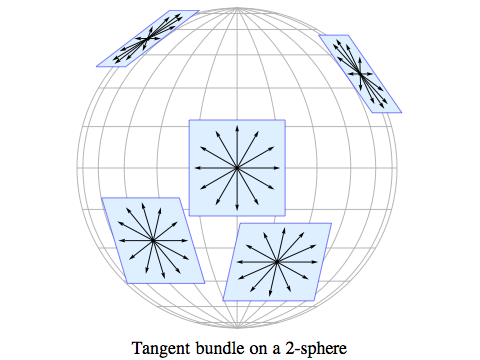
\includegraphics[scale=0.5]{tangent-bundle.png}
\end{equation}
\begin{equation}
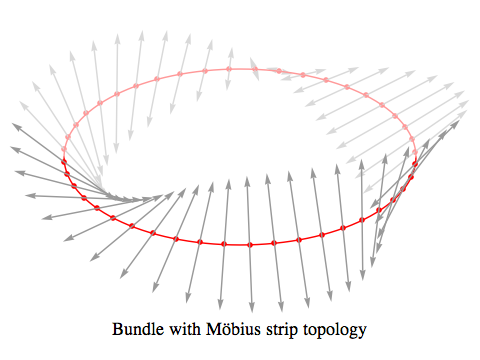
\includegraphics[scale=0.5]{tangent-bundle-2.png}
\end{equation}

粗略地,tangent bundle 可以看成是 $M \times T_x M$,而 $M$ 和 $T_x M$ 的维数都是 $n$,所以 tangent bundle 的维数是 $2n$。 在力学上,\emp{cotangent bundle} 就是相位空间 $(\vect{x}. \vect{p})$ 的空间 (The phase space of a mechanical system is the cotangent bundle of its configuration space)。

\subsubsection{Push forward, pull back}

\subsubsection{Energy conservation, area form}

(Stephanie \S 4.4)

\subsubsection{Symmetry of Hamiltonian system, Lie groups}

Symplectic groups 是一些保存辛结构的变换 $T$ 的群:
\begin{equation}
\omega(T x, T y) = \omega(x, y) \quad \forall x, y \in V
\end{equation}
$V$ 是向量空间。 在 $V$ 上的 symplectic 变换的全体记作 $Sp(V)$。

\subsubsection{Momentum maps}

\subsection{动态系统理论}

\subsubsection{Floer homology}

\emp{Homology (同调论)} 研究的是空间中「有没有穿洞」的樸拓结构。 最简单的 \emp{singular homology} 是将空间用三角形剖分 (triangulation),然后透过著名的 Euler formula $V + F = E + 2$ 及其扩充,让我们可以计算 Euler characteristic $\chi$,此即空间穿洞的个数。
\begin{equation}
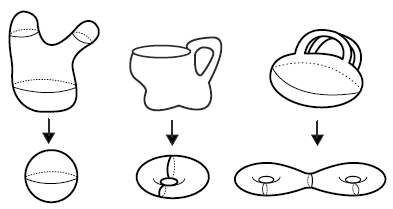
\includegraphics[scale=0.5]{manifolds-with-holes.png}
\end{equation}

\begin{equation}
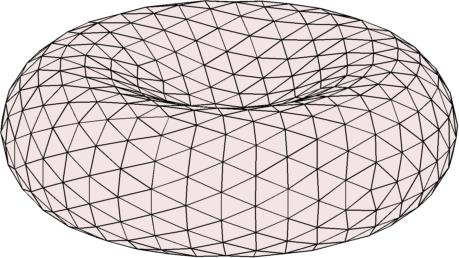
\includegraphics[scale=0.25]{torus-triangulation.jpg}
\end{equation}
当这些三角形剖分趋於无穷小时,我们得到用微分形式 (differential forms) 描述的 homology,即 \emp{de Rham homology}。 

\begin{equation}

\includegraphics[scale=0.5]{height-function.png}
\end{equation}
在流形上定义一个 potential function,例如简单的 height function,就可以做 Morse theory,这时每个点可以根据势能函数向下流 (gradient flow),流到一些最低位置,它们是临界点 (critical points)。 Morse decomposition 将空间用这些临界点分割(流到同一临界点的 flows 认作同一 equivalent class),得到的是 \emp{Morse homology}。
\begin{equation}
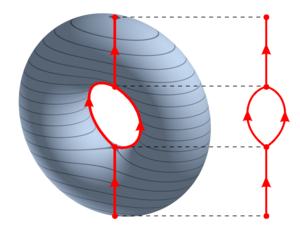
\includegraphics[scale=0.5]{gradient-flow.png}
\end{equation}

\emp{Floer homology} 是 Morse homology 的\textbf{无限维空间}版本,比较难计算。

\subsubsection{Conley theory}

\subsubsection{Entropy, ergodicity}

\subsubsection{Lie algebra 的另一应用}

例如一架车可以有两个基本动作: (A) 绕中心旋转、或 (B) 前后行驶,它们的 Lie 括号 $[A,B]$,产生出的动作是左右方向行驶,这类似於「平行泊车」的时候,车子的移动方向:
\begin{equation}
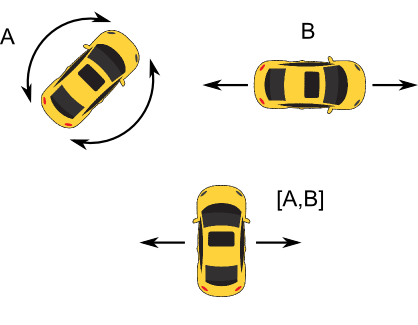
\includegraphics[scale=0.5]{Lie-bracket-car.png}
\end{equation}

(可控性与 ``reachable'' 概念。)

\subsubsection{Stable, unstable, and center manifold}

\subsubsection{Smale horseshoe}

\section{最优控制的计算方法}

\subsubsection{直接法}

\subsubsection{间接法}

\subsubsection{Lyapunov 函数第一方法}

\subsubsection{Lyapunov 函数第二方法}

\bibliographystyle{plain} % or number or aaai ...
\bibliography{AGI-book}

\end{document}
